%SourceDoc ../YourName-Dissertation.tex
\vspace*{-80mm}
\chapter{Isokinetic Sine Wave Advection} \label{chapter6:verification_1}
	    
The procedures that can be used for code verification, from least to most
rigorous, include: expert judgment, error quantification,
consistency/convergence, and order of accuracy \cite{Oberkampf2008}. For this
work, the Richardson extrapolation will be used to check for convergence and
order of accuracy of the error in space and time. The error should converge to
zero, and the order of accuracy should converge to the 1 as obtained through
the modified equation analysis in section \ref{Verification:MEA}.
 
\section{Problem Setup}

%Round off error, iterative convergence error.
%Discretization error?? (Check with)

To obtain an analytical solution for a subchannel code, typically the method
of manufactured solutions \cite{SAND2000-1444} is needed. To readily obtain an
analytical solution and isolate only the mass and energy conservation equations,
several simplifications to the verification problem are made. Only one channel
is considered to make the problem 1-D. In order to make the problem perfectly
isobaric and isokinetic, grid spacer losses, frictional losses, and gravity head
losses are set to zero representing a smooth horizontal pipe. Small fluctuations
in pressure and velocity may still occur due to the assumption that the EOS is
linear. The channel geometry and operating conditions approximate a standard PWR
as shown in table \ref{table:parameters}. The inlet of the channel has a
constant velocity with a fluctuating enthalpy that corresponds to be near the
standard PWR rod bundle coolant channel inlet conditions. The problem will aslo
have constant axial spacing and time step size. The length of the
transient was defined to be quadruple the time needed for the liquid at the
inlet to advect to the outlet. The frequency of the sine wave was defined to
generate a full period of a spatial wave across the length of the channel. With
these simplifications, the method of manufacturing solutions is unnecessary
since the known solutions are simply the advection of the transient inlet
conditions. The functions for the enthalpy $h$ and mass flow rate, $\dot{m}$,
are given in equations \ref{eq:Sine_Wave:h} and \ref{eq:Sine_Wave:m_dot} where
$x$ is the length from the inlet and $t$ is the simulated time. The functions
smoothly transition to the initial condition of a straight line across the
domain. The enthalpy and mass flow rate vary proportionally to the density such
that an isokinetic boundary condition is created at the inlet. While these
simplifications do not model a realistic problem, they appropriately isolate the
1-D single phase mass and energy conservation equations for the purpose of
verification. 

\begin{table}[h]
\center
\caption{Problem Parameters}
\label{table:parameters}
\begin{tabular}{|c|c|c|c|}
\hline
Parameter	&	Symbol	&	Value	&	Unit	\\ \hline
Axial Length	&	$L$	&	3.6586	&	$m$	\\ \hline
Channel Area	&	$A_{ch}$	&	4.94E-005	&	$m^{2}$	\\ \hline
Wetted Perimeter	&	$P_{w}$	&	1.49E-002	&	$m$	\\ \hline
Velocity	&	$V_{o}$	&	7.35	&	$\frac{m}{s}$	\\ \hline
Pressure	&	$P_{o}$	&	155.00	&	bar	\\ \hline
Temperature 1	&	$T_{1}$	&	289.500	&	$^{\circ}$C	\\ \hline
Temperature 2	&	$T_{2}$	&	327.00	&	$^{\circ}$C	\\ \hline
Enthalpy 1	&	$h_{1}$	&	1281.55	&	$\frac{kJ}{kg}$	\\ \hline
Enthalpy 2	&	$h_{2}$	&	1497.21	&	$\frac{kJ}{kg}$	\\ \hline
Mass Flow Rate 1	&	$\dot{m}_{1}$	&	0.2713	&	$\frac{kg}{s}$	\\ \hline
Mass Flow Rate 2	&	$\dot{m}_{2}$	&	0.2399	&	$\frac{kg}{s}$	\\ \hline
Final Time	&	$t_{f}$	&	2.00	&	sec	\\ \hline
Wave Frequency	&	$\omega$	&	1.00	&	Hz	\\ \hline
\end{tabular}
\end{table}

\begin{equation}
	\label{eq:Sine_Wave:h}
	h(i,j) = \frac{1}{2} \left( 
			(h_{1}+h_{2}) + (h_{1}-h_{2}) cos\left(
				\omega \left( j \Delta t + \frac{i \Delta x}{V_{o}} \right)
				\right)
			\right)
\end{equation}

\begin{equation}
	\label{eq:Sine_Wave:m_dot}
	\dot{m}(i,j) = \frac{1}{2} \left( 
			(\dot{m}_{1}+\dot{m}_{2}) + (\dot{m}_{1}-\dot{m}_{2}) cos\left(
				\omega \left( j \Delta t + \frac{i \Delta x}{V_{o}} \right)
				\right)
			\right)
\end{equation}

The comparison between the data table and the output in CTF are shown for
enthalpy and mass flow rate in figures \ref{fig:Inlet_h} and
\ref{fig:Inlet_m_dot}, respectively. The CTF output was read from the high
precision VTK data files \cite{Schroeder1998} at each point in time, which
omitted the actual ghost cell where these values were applied. The CTF values are located at the nearest
node to the inlet, and will experience small amounts of numerical diffusion. For
large mesh sizes, this discrepancy is negligible as can be seen by the
overlapping profiles in figures \ref{fig:Inlet_h} and \ref{fig:Inlet_m_dot}.

\begin{figure}[!h]
	\centering
	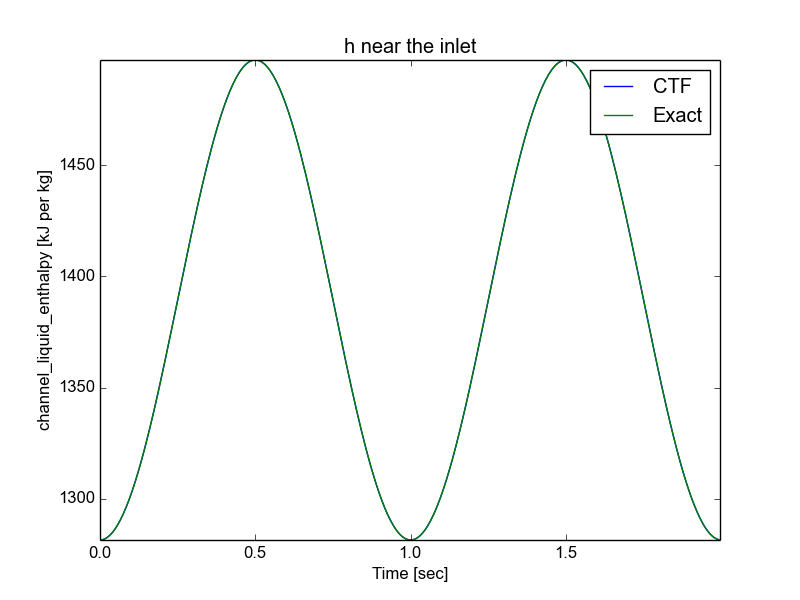
\includegraphics[width=0.55\textwidth]{images/Code_Verification/run_00_00/residual/results/Inlet_h.png}
	\caption{Enthalpy Near the Inlet and the Analytical Solution}
	\label{fig:Inlet_h}
\end{figure}

\begin{figure}[!h]
	\centering
	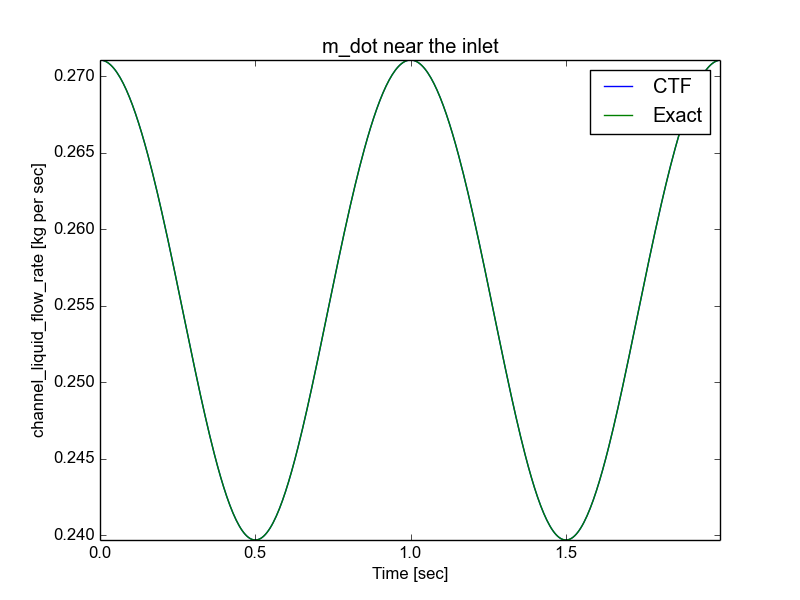
\includegraphics[width=0.55\textwidth]{images/Code_Verification/run_00_00/residual/results/Inlet_m_dot.png}
	\caption{Density Near the Inlet and the Analytical Solution}
	\label{fig:Inlet_m_dot}
\end{figure}

% For the original version of CTF, there is a small discrepancy in the way the
% density is calculated at the inlet that causes the velocity to be non-constant.
%as shown in figure \ref{fig:Inlet_vel}.
 The pressure and the velocity fluctuate by less than $0.25\%$ during the
 simulation due to approximating the EOS as a linear function. This is considered small for
 this problem and should not greatly affect the order of accuracy of the error. 
 The VTK output files allow for a high level of precision, reducing
 round off error in the output during the post processing.

\section{Code Convergence}

The current version of CTF uses global code convergence criteria that are
used to estimate the rate of change of global mass and energy conservation. The
transient values of these criteria are shown in figure \ref{fig:Code_Convergence:Original} for the original version of
CTF simulating the verification problem. Mass balance and storage are in units
of $\frac{kg}{s}$. The energy balance, fluid energy, and solid energy are in units of $kW$.
The solid energy storage is zero since there are not any heat structures present. The fluctuating values
represent differences between the energy and mass entering and leaving the
system. The flat profile for the mass storage term means that the sine wave has
fully developed spatially through the channel. 

\begin{figure}[!h]
	\centering
	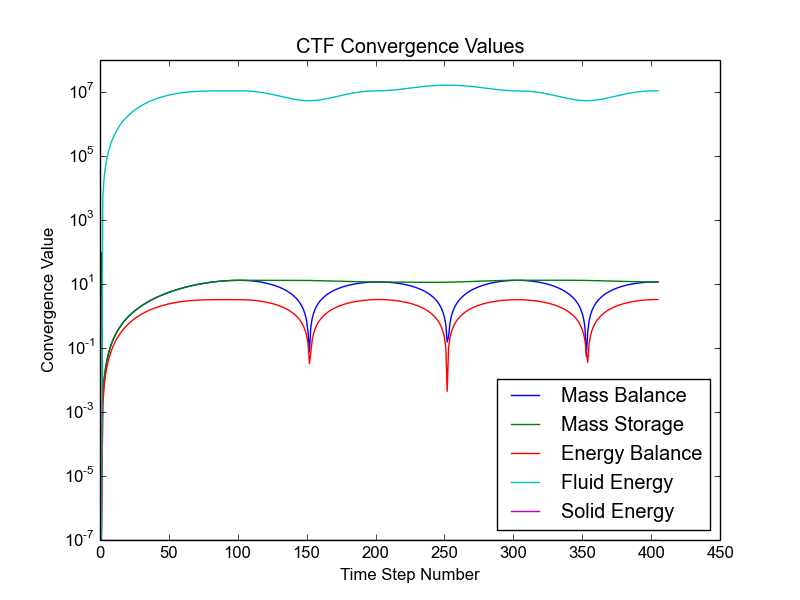
\includegraphics[width=0.50\textwidth]{images/Code_Verification/run_00_00/original/results/Convergence_Plot.png}
	\caption{Code Convergence Criteria for the Original Version of CTF}
	\label{fig:Code_Convergence:Original}
\end{figure}

\begin{figure}[!h]
	\centering
	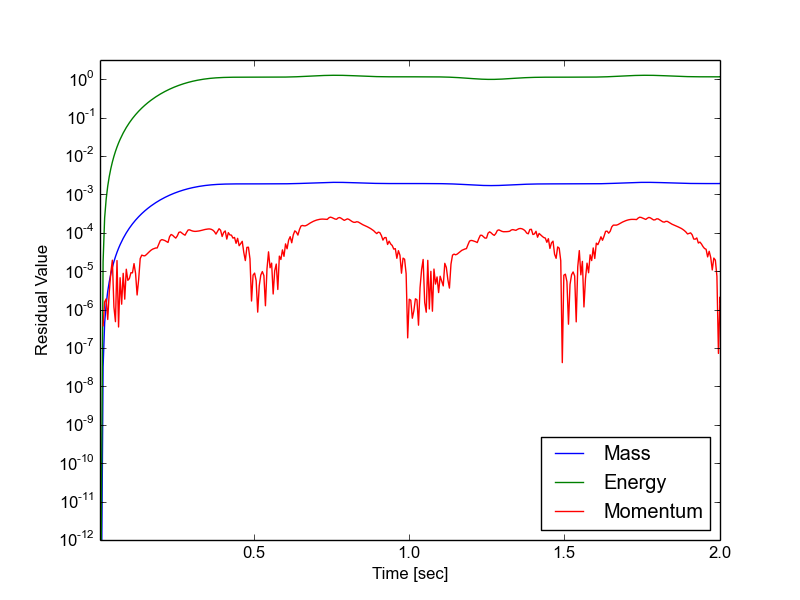
\includegraphics[width=0.50\textwidth]{images/Code_Verification/run_00_00/residual/results/Residuals_Plot.png}
	\caption{Summation of the Residuals for the Residual Version of CTF}
	\label{fig:Residuals_Plot}
\end{figure}

The residual formulation prints out the summation of the equation residuals
across the domain to an output file at the end of each time step and can be seen
in figure \ref{fig:Residuals_Plot}. The mass equation residual is in units of
$\frac{kg}{m^{3}s}$. The energy equation residual is in units of
$\frac{kW}{m^{3}}$. The momentum residual is in units of
$\frac{kg}{m^{2}s^{2}}$. The flat profile of the mass and energy residuals shows
that the sine wave has fully developed spatially through the channel.

\section{Richardson Extrapolation}

The Richardson extrapolation was performed by refining the spatial and temporal
step sizes by a factor of 2 for a set number of times. The spatial and temporal
studies are refined separately in their own study in order to isolate the
spatial and temporal affects on the solution. The generation of the inputs,
running of the codes, and analysis of the output were automated with a python
\cite{python} script in order to reduce user input errors and increase
repeatability. For this analysis, a significant amount of information was added
to the VTK output files, increasing memory usage and run time. The computational
resources for the spatial study was much higher than the temporal study due to
the need to keep the CFL number below 0.500. To keep the computational resources
needed to perform this analysis reasonable, fewer spatial refinements were
performed compared to the temporal analysis.

\section{Convergence of Error}

The difference between iterations was computed at each time step and spatial
location for each quantity of interest. This difference is considered as the
error between each iteration. For the spatial refinement, the lower iterate
values were numerically integrated to match the shape of the initial domain. The
errors were then summed over the entire domain to yield a total error for each
variable. The total error for density is plotted in figures
\ref{fig:Temporal:Diff_rho} and \ref{fig:Spatial:Diff_rho} as a function of
temporal and spatial step size.

\begin{figure}[!h]
	\centering
	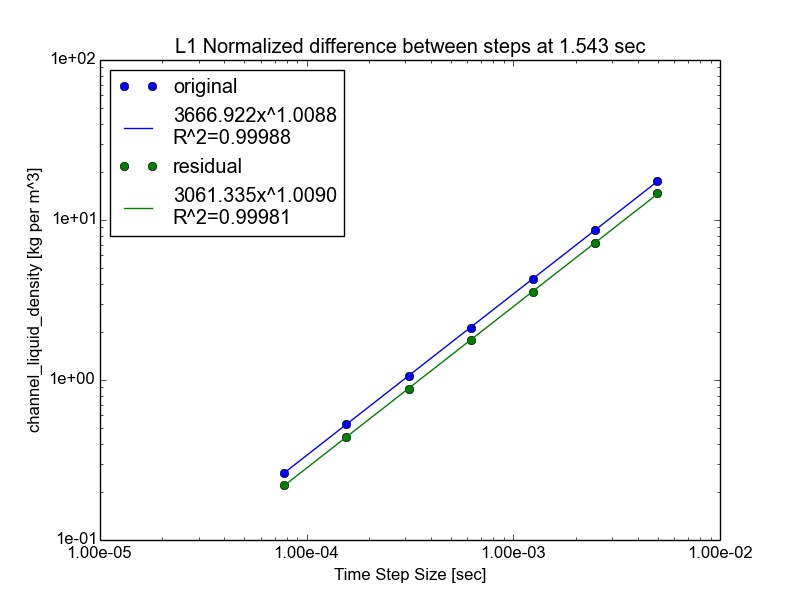
\includegraphics[width=0.60\textwidth]{images/Temporal_Study/Difference_rho}
	\caption{Difference Between Successive Temporal Refinements for Density}
	\label{fig:Temporal:Diff_rho}
\end{figure} 

The data points were chosen to be inside of the asymptotic range as shown by
the good power fit with an exponent near 1. The power fit shows that as the
temporal and spatial step sizes are reduced, the numerical error approaches
zero. The discretization error between the original version of CTF is
relatively small and is most likely due to the small fluctuations in the
velocity present in the original version of the code. 

\begin{figure}[!h]
	\centering
	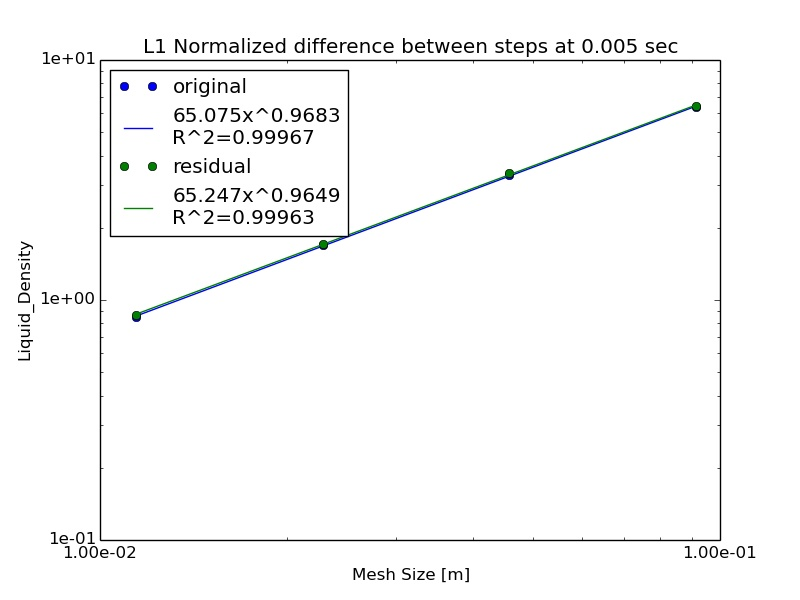
\includegraphics[width=0.60\textwidth]{images/Spatial_Study/Difference_rho}
	\caption{Difference Between Successive Spatial Refinements for Density}
	\label{fig:Spatial:Diff_rho}
\end{figure} 

\section{Order of Accuracy}

The order of accuracy for this verification problem is first order as shown by
the modified equation analysis. This can be considered to be the exponent on
the power fits as seen in figures \ref{fig:Temporal:Diff_rho}. However the order
of accuracy $p$ can be calculated by using equation \ref{eq:OOA} where $f_{1}$,
$f_{2}$, $f_{3}$ are consecutive levels within the same Richardson extrapolation
study. The refinement factor, $R$, has the constant value of 2 for both the
spatial and temporal studies.

\begin{equation}
	\label{eq:OOA}
	p= \frac{
	      	ln \left(
	      	\frac{f_{3}-f_{2}}{f_{2}-f_{1}}
	      	\right)
	    }{ln(R)}
\end{equation}

The order of accuracy for all of the variables are presented for the temporal
analysis and spatial analysis in figures \ref{fig:Temporal:OOA} and
\ref{fig:Spatial:OOA} respectively. The temporal order of accuracy is well
within the asymptotic range for the whole analysis, and moves closer to 1.0 with
decreasing time step size. The spatial order of accuracy is a slightly outside
the asymptotic range, but approaches an order of accuracy of 1.0 with
decreasing mesh size. 

\begin{figure}[!h]
	\centering
	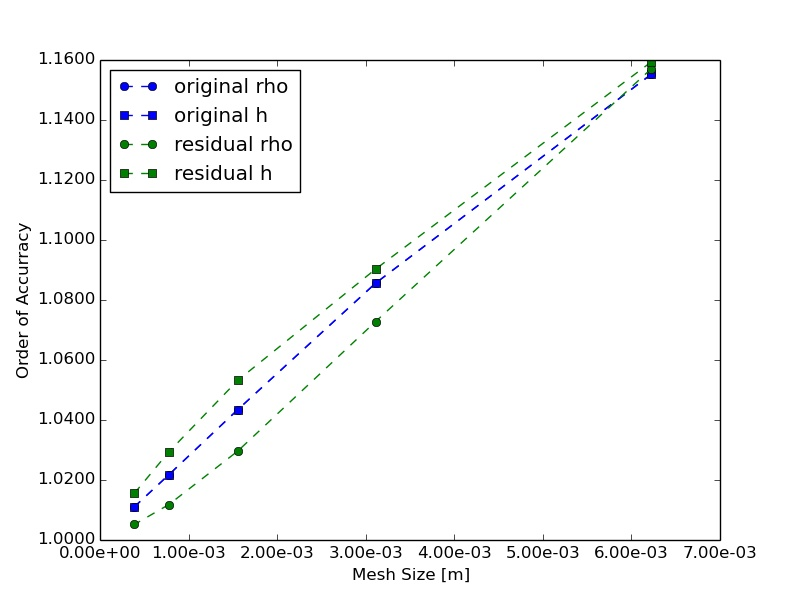
\includegraphics[width=0.60\textwidth]{images/Temporal_Study/Order_Of_Accuracy_Summary}
	\caption{Temporal Order of Accuracy}
	\label{fig:Temporal:OOA}
\end{figure}

The slight differences between the original version of CTF and the residual
formulation might be due to the different solution methods and back substitution
of variables. Despite the small differences, both versions of the code exhibit
order of accuracies very close the values obtained through the modified
equation analysis.

\begin{figure}[!h]
	\centering
	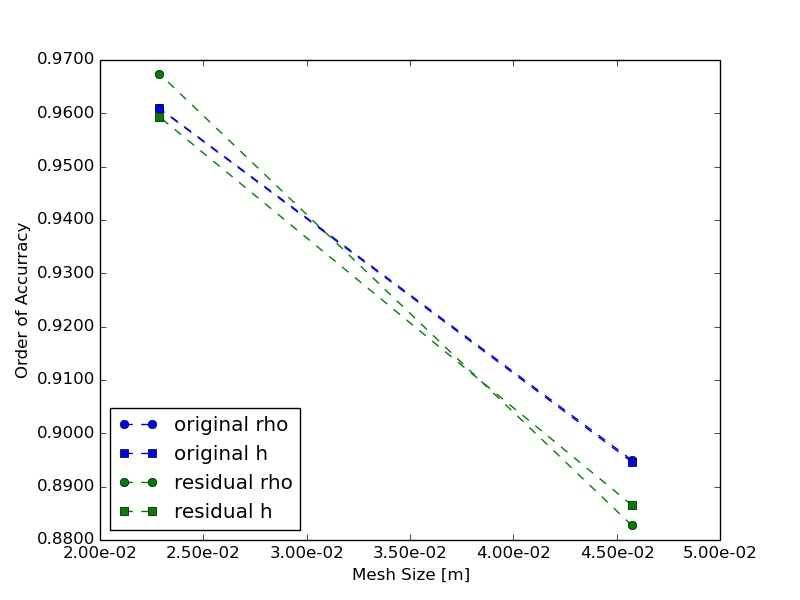
\includegraphics[width=0.60\textwidth]{images/Spatial_Study/Order_Of_Accuracy_Summary}
	\caption{Spatial Order of Accuracy}
	\label{fig:Spatial:OOA}
\end{figure}

Taking the derivative of the analytical solution, the exact numerical error can
be calculated from the modified equation analysis and compared to the
calculated error as seen in figure \ref{fig:Error_comparison_rho}. This error
was scaled by a factor of $\frac{x}{L}$ to account for numerical propagation.
The temporal and spatial mesh sizes were selected to have order of accuracies
that were closest to 1. There still exists a small discrepancy between the
expected error, and the calculated error. However, this is small enough that it
is most likely due to truncation error in either the solution of the Jacobian
matrix or in values read in from CTF. 

\begin{figure}[!h]
	\centering
	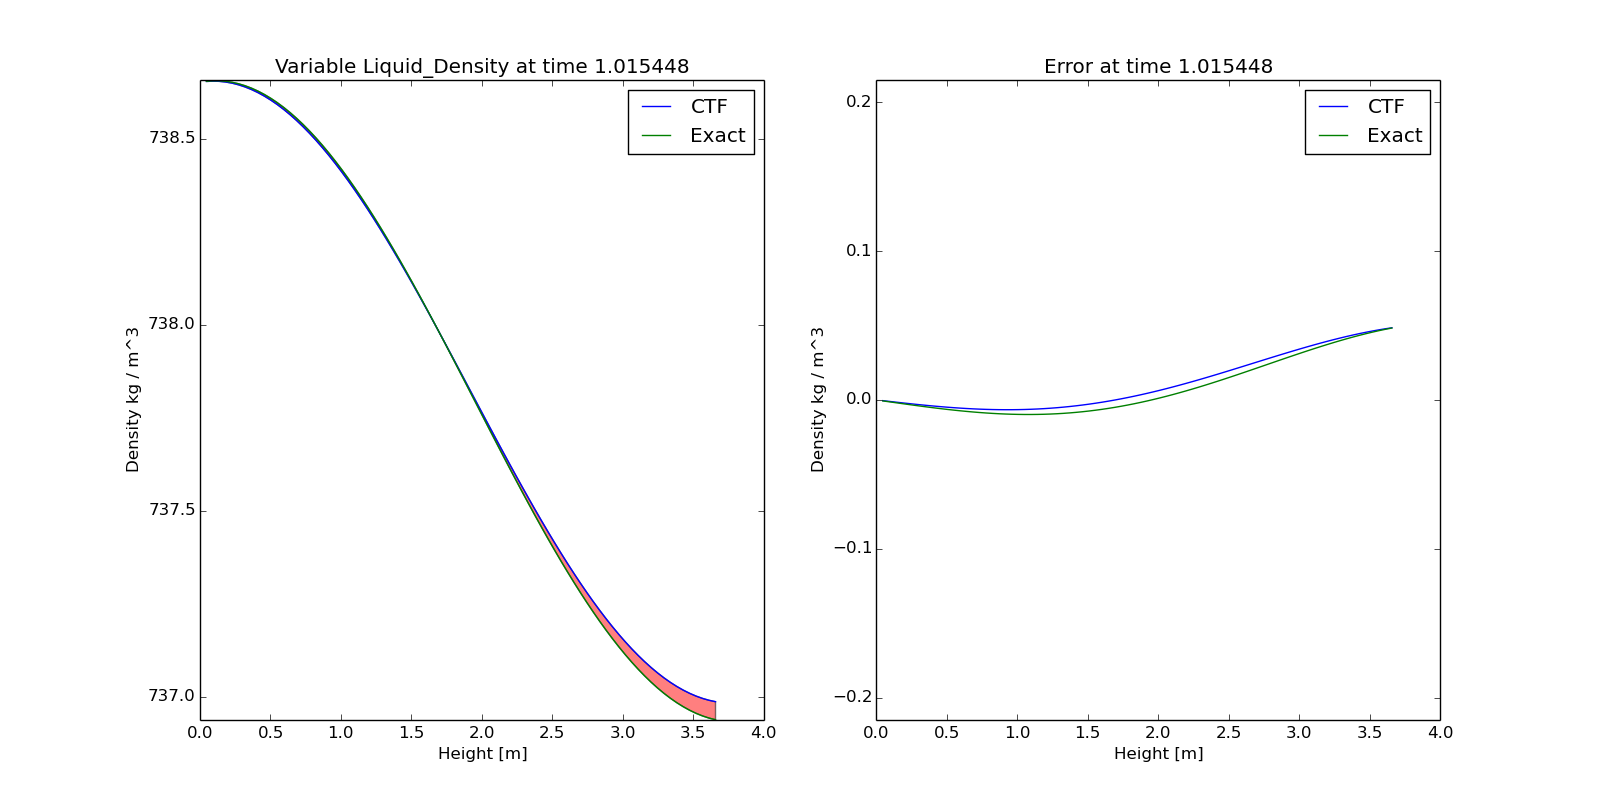
\includegraphics[width=1.00\textwidth]{images/Error_comparison_rho.png}
	\caption{Comparison of the Error for Density}
	\label{fig:Error_comparison_rho}
\end{figure}






